In order to better understand the algorithm, and to test its effectiveness, I created my own implementation. I used \textbf{Successive Over-Relaxation} as opposed to Gauss-Seidel, since this exhibited better results (SOR is the same as Gauss-Seidel, except that after solving for the error and interpolating, the result is multiplied by a user chosen value between 0 and 2). I also used a variant on the Matting Laplacian from \cite{levin08} that takes into account the RGB channels of the image, rather than just the grayscale intensity at each pixel. I used the interpolation and restriction operators described in \cite{lee14}, as well as the V-Cycle algorithm for multigrid. Since speed was an important factor in testing my implementation, I chose to write it in C++ (a decision made also by the authors of \cite{lee14}).
\\\\
In general, my results were quite impressive. My implementation does not exhibit convergence as rapidly as \cite{lee14}, so I believe there may still be errors in the code, but this does not prevent most images from converging to fairly accurate mattes. One of the most prominent features of this method is just how much of a different the multigrid optimization makes. Consider the following image and sketch:
\\
\begin{center}
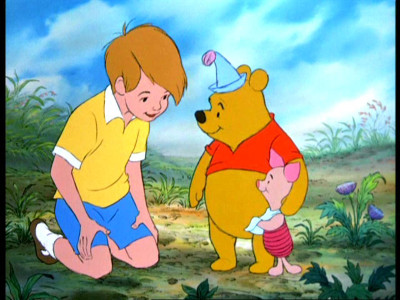
\includegraphics[width=2.2in]{fig/pooh_med.jpg}
\hspace{.2in}
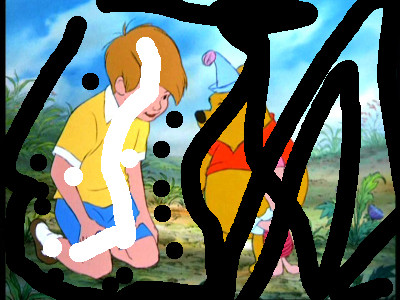
\includegraphics[width=2.2in]{fig/christopher_med_sketch.jpg}
\end{center}
The following images were both produced with 50 iterations of SOR, but the first did not have multigrid steps enabled, while the second did. The difference is startling!
\\
\begin{center}
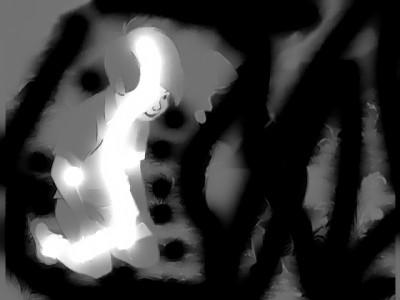
\includegraphics[width=2.2in]{fig/christopher_med_result_nogrid.jpg}
\hspace{.2in}
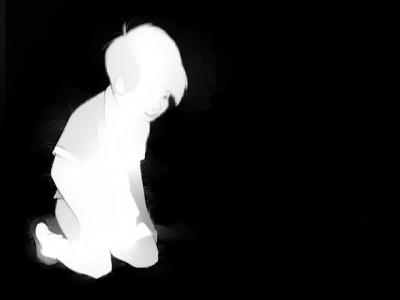
\includegraphics[width=2.2in]{fig/christopher_med_result.jpg}
\end{center}
This difference is just as pronounced on other images. Clearly relaxation has similar problems on images as it did on the sample problem earlier explained! In the second image, it's apparent that there are issues with matting around the edges of the image. Although this is likely mostly an implementation issue, I did notice that many of the images shown in papers used images with in-focus foregrounds and blurry, relatively uniform backgrounds. When applied to images of this type, my implementation also had quite impressive results. With 30 iterations, the following sketch produced an excellent matte:
\\
\begin{center}
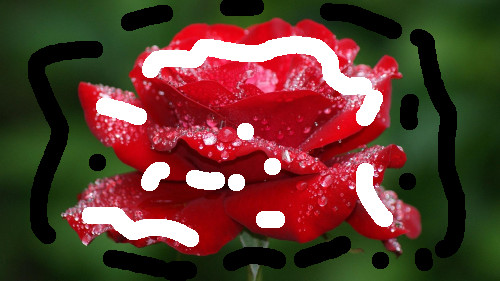
\includegraphics[width=2.2in]{fig/rose.jpg}
\hspace{.2in}
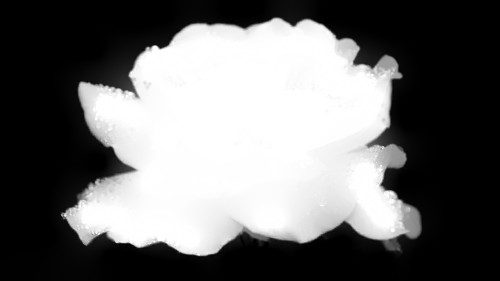
\includegraphics[width=2.2in]{fig/rose_result.jpg}
\end{center}
In instances such as this, the practical applications of image matting in simple image editing become quite apparent. Complex shapes can be cut out of images with minimal effort and high accuracy. When results are not satisfactory, adding a few lines to the sketch is almost always sufficient. For example, the above matte was used to produce the image below.
\\
\begin{center}
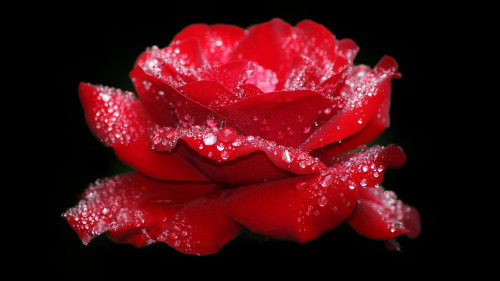
\includegraphics[width=4.6in]{fig/rose_blackbg.jpg}
\end{center}
With a bit of effort to produce a good sketch, very good mattes can be produced. However, one drawback of the strict constraints of the user sketch can become apparent on images with large semi-transparent regions. Consider the following matting application:
\\
\begin{center}
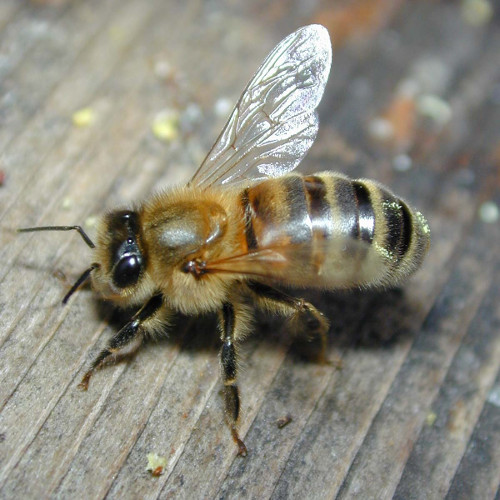
\includegraphics[width=2.2in]{fig/bee.jpg}
\hspace{.2in}
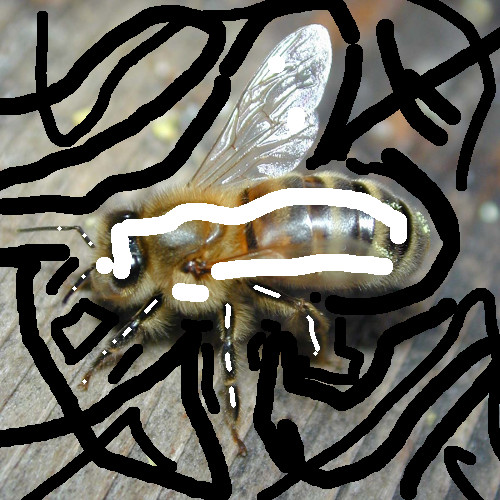
\includegraphics[width=2.2in]{fig/bee_sketch.jpg}
\end{center}
\begin{center}
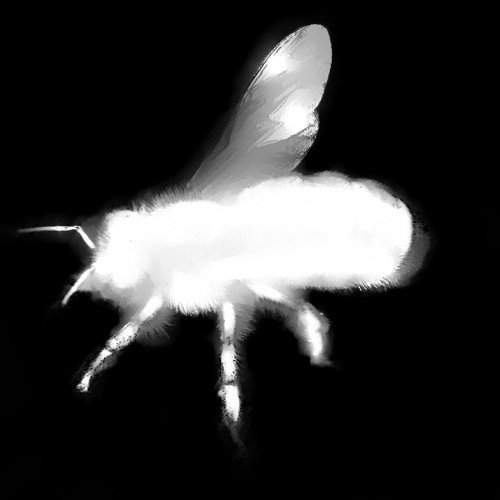
\includegraphics[width=2.2in]{fig/bee_result.jpg}
\hspace{.2in}
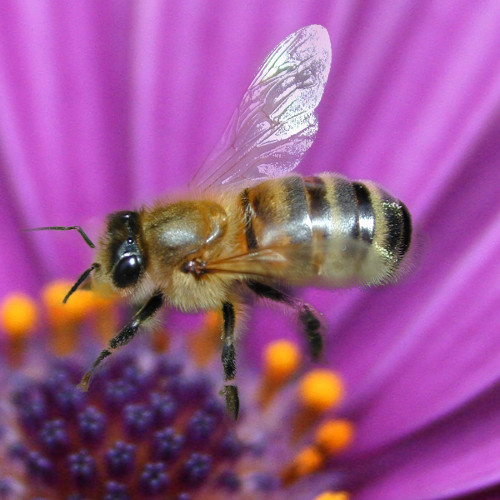
\includegraphics[width=2.2in]{fig/bee_on_flower.jpg}
\end{center}
The complex shape of the bee is selected very accurately withe the sketch given, but the wings are a problem. They are everywhere transparent, but any places marked as part of the foreground then become complete opaque. In the above matte, it is clear that the correct transparency was determined for most of the wing, but the places marked in the sketch are unnaturally white.
\\\\
The code for this implementation can be found at\\ \url{https://github.com/dylanswiggett/image-matting/tree/master/impl}.